\documentclass[../main.tex]{subfiles}
\begin{document}

    \begin{itemize}
        \item Wymagania to \textbf{opis funkcji} (usług) i ograniczeń dla systemu.
        \item Wymagania nie opisują jak system ma działać, a \textbf{co ma
        wykonywać}.
        \item Definiowane na \textbf{wczesnych etapach rozwoju} systemu jako specyfikacja tego, co ma być
        implementowane.
        \item Inżynieria wymagań to proces pozyskiwania, analizowania, dokumentowania oraz weryfikowania
        wymagań dla projektowanego systemu.

    \end{itemize}

    \subsection{Klasyfikacja wymagań}
    \begin{itemize}
        \item \textbf{Funkcjonalne} - czynność, zadanie.
        \item \textbf{Pozafunkcjonalne} - technikalia mierzone metrykami.
    \end{itemize}

    \textbf{Klasyfikacja wymagań - FURPS} - \textbf{F}unctionality, \textbf{U}sability, \textbf{R}eliability,
    \textbf{P}erformance, \textbf{S}ecurity.

    \subsubsection{Wymagania funkcjonalne - „System powinien\dots”}
    \begin{itemize}
        \item \textbf{Zalety}: łatwość spisywania,
        \item \textbf{Wady}: słaba czytelność, trudne sprawdzanie kompletności i spójności.
        \item \textbf{Przypadki użycia}:  łatwość spisywania, czytelność, łatwość zrozumienia; forma ustrukturalizowana.
        \item \textbf{Historyjki użytkownika} - Who? What? Why?
    \end{itemize}

    Cecha \textbf{INVEST}:
    \begin{itemize}
        \item \textbf{Independent} - zależności powodują problem z estymacją),
        \item \textbf{Negotiable},
        \item \textbf{Valuable},
        \item \textbf{Estimable},
        \item \textbf{Small} (jeden sprint),
        \item \textbf{Testable}.
    \end{itemize}

    \subsubsection{Wymagania pozafunkcjonalne}
    \begin{itemize}
        \item Ograniczenia usług lub funkcji, np. czasowe, procesu rozwoju oprogramowania, standardy.
        \item Każda cecha to \textbf{zbiór atrybutów}.
        \item Stanowią \textbf{niezbędne uzupełnienie wymagan funkcjonalnych} dla oprogramowania,
        \item Problemy z oprogramowaniem wskazują na silną potrzebę precyzyjnego definiowania atrybutów
        (charakterystyk) dla tworzonych produktów programistycznych.
    \end{itemize}


    \begin{table}[H]
        \begin{center}
            \begin{tabular}{  p{8cm} p{8cm} }
                \textbf{Niezawodność} - zdolność do spełnienia i utrzymania
                określonych wymagań stabilności, przy spełnieniu określonych
                warunków oraz w określonych ramach czasowych.
                &
                \begin{itemize}
                    \item Dojrzałość
                    \item Odporność na błędy
                    \item Zdolność do odtworzenia
                \end{itemize}
                \\

                \cmidrule(r){1-1}\cmidrule(l){2-2}

                \textbf{Wydajność} - opisuje powiązania miedzy poziomem wydajności oprogramowania, a
                wykorzystywanymi zasobami przy spełnieniu określonych warunków.
                &
                \begin{itemize}
                    \item Wykorzystanie czasu
                    \item Wykorzystanie zasobów
                \end{itemize}
                \\

                \cmidrule(r){1-1}\cmidrule(l){2-2}

                \textbf{Użyteczność} - opisuje nakład pracy niezbędny do swobodnego posługiwania się oprogramowaniem.
                &
                \begin{itemize}
                    \item Łatwość zrozumienia
                    \item Łatwość nauki
                    \item Operatywność
                \end{itemize}
                \\

                \cmidrule(r){1-1}\cmidrule(l){2-2}

                \textbf{Łatwość konserwacji} - opisuje nakład pracy niezbędny do wprowadzenia zmian do oprogramowania.
                &
                \begin{itemize}
                    \item Łatwość analizy
                    \item Łatwość wprowadzania zmian
                    \item Stabilność
                    \item Łatwość testowania
                \end{itemize}
                \\

                \cmidrule(r){1-1}\cmidrule(l){2-2}

                \textbf{Przenośność} - opisuje zdolność oprogramowania do przenoszenia między różnymi środowiskami/platformami.
                &
                \begin{itemize}
                    \item Łatwość adaptacji
                    \item Zgodność
                    \item Łatwość instalacji
                    \item Łatwość zastąpienia
                \end{itemize}
                \\


            \end{tabular}
        \end{center}
    \end{table}

    \subsection{Analiza wymagań/analiza obiektowa}
    \begin{itemize}
        \item Celem jest stworzenie modelu systemu, zwanego \textbf{modelem analitycznym}.
        \item Wysiłek uczestników projektu skupia się na strukturalizowaniu i formalizowaniu zabranych
        wcześniej wymagań.
    \end{itemize}

    \begin{table}[H]
        \begin{center}
            \begin{tabular}{ c p{8cm} }
                \raisebox{-\totalheight}{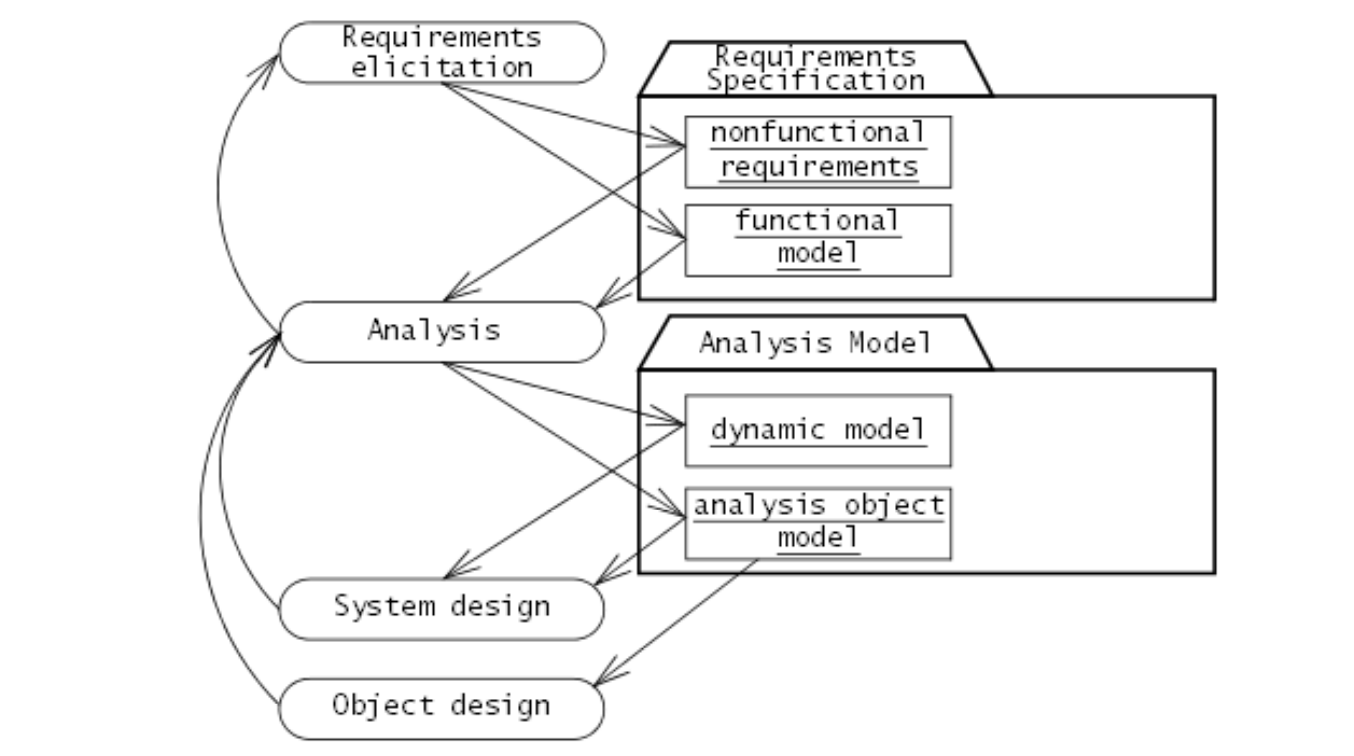
\includegraphics[width=0.5\textwidth]{analiza_wymagan.png}}
                &
                \begin{itemize}
                    \item \textbf{Model analityczny} – reprezentuje tworzony system z perspektywy użytkownika; opis co system powinien robić.
                    \item \textbf{Analityczny model obiektowy} – odzwierciedla indywidualne koncepcje korzystania z systemu, ich właściwości i relacje między nimi (diagramy klas).
                    \item \textbf{Model dynamiczny} - koncentruje się na zachowaniu systemu(diagramy sekwencji i stanów).
                    \item \textbf{Obiekty encji} – reprezentują trwałą informację potwarzaną przez system.
                    \item \textbf{Obiekty brzegowe} – odzwierciedlają interakcje między aktorami a systemem.
                    \item \textbf{Obiekty sterujące} – odpowiedzialne są za realizację przypadków użycia.
                    \item \textbf{Relacja dziedziczenia} umożliwia hierarchiczne organizowanie koncepcji.
                    \item \textbf{Generalizowanie} - aktywność identyfikowania abstrakcyjnych koncepcji na podstawie przykładów i konkretyzacji.
                    \item \textbf{Specjalizowanie} - aktywność odwrotna, czyli identyfikowanie koncepcji bardziej specyficznych na podstawie koncepcji wysokopoziomowej.
                \end{itemize}
                \\
            \end{tabular}
        \end{center}
    \end{table}


\end{document}